\documentclass[a4paper, 12pt]{article}

% Русский язык
\usepackage[T2A]{fontenc}
\usepackage[utf8]{inputenc}
\usepackage[english,russian]{babel}

% Картинки
\usepackage{graphicx}
\graphicspath{{images/}}
\DeclareGraphicsExtensions{.pdf,.png,.jpg}
\usepackage{wrapfig}

% Математика
\usepackage{amsmath,amsfonts,amssymb,amsthm,mathtools} 

% Параметры страницы
\usepackage[left=2cm,right=2cm,top=2cm,bottom=3cm,bindingoffset=0cm]{geometry}

\usepackage{enumitem,xparse}
\usepackage{caption}
\usepackage{subcaption}
\usepackage{float}

\begin{document}

\newgeometry{left=2cm,right=2cm,top=2cm,bottom=1cm,bindingoffset=0cm}
\begin{titlepage}
    
    \begin{center}
        \vspace*{5cm}
        \Huge Московский Физико-Технический Институт
        \vspace*{2cm}\\
        \LARGE Отчет по эксперименту
        \\\vspace*{0.25cm}
        
        \noindent\rule{\textwidth}{1pt}
        \vspace*{-0.25cm}
        
        \huge \textbf{1.1.4\\ Изучение статистических закономерностей на примере измерения фона космического излучения}
        \noindent\rule{\textwidth}{1pt}


       \vfill
        \begin{flushright}
            \begin{minipage}{.4\textwidth}
            \Large Выполнил:\\ Студент 1 курса ФАКТ\\ Группа Б03-504 \\Подмосковнов Лев\\
            \end{minipage}
        \end{flushright}
        
        \vfill
        \normalsize Долгопрудный \\2025
        
    \end{center}
\end{titlepage}
\restoregeometry

\setcounter{page}{2}
\section*{Аннотация}
\noindent \textbf{Цель работы:} на примере статистики регистрации фоновых космических частиц изучить статистические закономерности однородного во времени случайного процесса; проверить возможность описания исследуемого процесса статистическими законами Пуассона и Гаусса; измерить среднее число регистрируемых космических лучей в секунду и определить погрешность результата.

\noindent \textbf{В работе используются:} счётчик Гейгера—Мюллера, компьютер с интерфейсом для связи со счётчиком, расчётная программа.

\section*{Базовые теоретические понятия}

Далее будем для простоты считать, что все прочие погрешности, помимо статистических, пренебрежимо малы и рассматривать их не будем. В рамках нашего опыта это предположение хорошо выполняется.

Наиболее важной характеристикой является выборочное среднее значение числа измерений.
\[\langle n \rangle=\frac{1}{n}\sum^{N}_{i=1}n_{i}\]

Если продолжать проводить измерения, можно ожидать, что выборочное среднее будет стремиться к некоторому конечному пределу, который можно назвать «истинным» средним значением числа регистрируемых частиц.
\[\overline n = \lim_{N \to \infty} \langle n \rangle\]

Кроме среднего значения важно знать, насколько сильно флуктуируют
значения $n_{i}$ от опыта к опыту. Количественно меру флуктуаций принято измерять среднеквадратичным (или стандартным) отклонением $\sigma_{n}$. По определению, средний квадрат отклонения, называемый также дисперсией.
\[\sigma^2_{n}\equiv\frac{1}{N}\sum_{i}^{N}(n_{i}-\langle n\rangle)^2\]

Короче будет так
\[\sigma^2_{n}\equiv\langle n_{i}-\langle n\rangle\rangle^2\]

Аналогично, при $N \to \infty$ выборочная дисперсия должна стремиться к некоторому предельному («истинному») значению:
\[\overline{\sigma}^{2}= \lim_{N \to \infty} {\sigma}^{2}_{n}=\overline{(n-\overline{n})^{2}}\]

Погрешность среднего значения $\langle n \rangle$ при независимых измерениях связана со
стандартным отклонением (погрешностью отдельного измерения) формулой
\begin{equation}\label{average}
    \sigma_{\langle n \rangle}=\frac{\sigma_{n}}{\sqrt{N}}
\end{equation}

\vspace{2cm}

Таким образом, если среднеквадратичное отклонение  $\sigma_{n}$ стремится к конечному пределу при больших $N$ погрешность среднего значения убывает с ростом числа измерений как $\frac{1}{\sqrt{N}}$ Иными словами, увеличивая количество измерений, среднее значение можно получать со всё более возрастающей точностью, приближаясь к «истинному» $\overline{n}$. А при конечном $N$ можно записать,
что истинное среднее с высокой вероятностью лежит в интервале
\[\overline{n}=\langle n\rangle \pm \frac{\sigma_{n}}{\sqrt{N}}\]

\subsection*{Пуассоновский процесс}
 
Вероятности $w_{n}$ того, что в эксперименте будет обнаружено $n$ частиц, для
распределения Пуассона имеют вид
\[w_{n}=\frac{\overline{n}^{n}}{n!}e^{-\overline{n}}\]\

Наиболее характерным свойством распределения Пуассона является связь между его дисперсией и средним значением. А именно, для пуассоновского процесса (и только для него!) справедливо равенство
\begin{equation}\label{puason}
    \sigma=\sqrt{\overline{n}}    
\end{equation}

На практике можно ожидать приближённое равенство для выборочных значений:
\[\sigma_{n}\approx\sqrt{\langle n\rangle}\]

\subsection*{Погрешность эксперимента}
Подставим основное свойство распределения Пуассона \eqref{puason} в формулу \eqref{average}. Получим среднеквадратичную погрешность определения среднего:
\[\sigma_{\langle n\rangle}=\frac{\sigma_{n}}{\sqrt{N}}=\sqrt{\frac{\langle n \rangle}{N}}\]

Обычно больший интерес представляет не абсолютное, а относительное значение погрешности. Для него находим:
\[\varepsilon_{n}=\frac{\sigma_{\langle n\rangle}}{\langle n\rangle}=\frac{1}{\sqrt{\langle n\rangle N}}=\frac{1}{\sqrt{n_{\Sigma}}}\]

\section*{Выполнение задания}

Сгруппируем и просуммируем соседние данные с различными интервалами группировки: $\tau$ = 10 с; 20 с; 40 c; 80c 

\vspace{5cm}
\subsection*{При $\tau=10 c$}

\begin{table}[!h]
\begin{center}
\begin{tabular}{|c|c|c|c|c|c|c|c|c|c|c|}
\hline
№Опыта & 1 & 2 & 3 & 4 & 5 & 6 & 7 & 8 & 9 & 10 \\ \hline 
0 & 12 & 10 & 10 & 10 & 19 & 8  & 6  & 11 & 7  & 17 \\ \hline
10 & 11 & 10 & 8  & 10 & 10 & 11 & 15 & 9  & 12 & 14 \\ \hline
20 & 11 & 10 & 17 & 10 & 11 & 13 & 10 & 13 & 9  & 15 \\ \hline
30 & 10 & 10 & 11 & 10 & 10 & 12 & 9  & 14 & 13 & 9  \\ \hline
40 & 9  & 9  & 9  & 10 & 8  & 15 & 12 & 13 & 12 & 8  \\ \hline
50 & 12 & 12 & 22 & 14 & 18 & 15 & 13 & 14 & 13 & 14 \\ \hline
60 & 15 & 20 & 9  & 8  & 16 & 10 & 17 & 15 & 11 & 13 \\ \hline
70 & 9  & 14 & 14 & 9  & 8  & 8  & 3  & 14 & 12 & 10 \\ \hline
80 & 8  & 13 & 12 & 19 & 8  & 10 & 14 & 6  & 12 & 8  \\ \hline
90 & 10 & 19 & 12 & 9  & 16 & 11 & 12 & 12 & 11 & 15 \\ \hline
100 & 12 & 9  & 12 & 8  & 16 & 17 & 18 & 6  & 12 & 15 \\ \hline
110 & 13 & 14 & 15 & 15 & 18 & 16 & 16 & 14 & 10 & 12 \\ \hline
120 & 14 & 16 & 14 & 11 & 8  & 10 & 13 & 15 & 9  & 13 \\ \hline
130 & 11 & 6  & 9  & 8  & 15 & 10 & 13 & 12 & 11 & 20 \\ \hline
140 & 14 & 17 & 18 & 10 & 7  & 7  & 14 & 14 & 16 & 13 \\ \hline
150 & 16 & 11 & 16 & 14 & 12 & 12 & 14 & 10 & 6  & 13 \\ \hline
160 & 14 & 13 & 12 & 19 & 15 & 14 & 11 & 20 & 12 & 10 \\ \hline
170 & 11 & 12 & 14 & 14 & 16 & 14 & 15 & 14 & 10 & 8  \\ \hline
180 & 9  & 9  & 14 & 10 & 13 & 12 & 9  & 11 & 11 & 13 \\ \hline
190 & 9  & 10 & 14 & 6  & 10 & 15 & 12 & 11 & 18 & 14 \\ \hline
200 & 7  & 9  & 12 & 13 & 12 & 8  & 9  & 16 & 9  & 12 \\ \hline
210 & 19 & 15 & 11 & 20 & 17 & 6  & 14 & 10 & 10 & 19 \\ \hline
220 & 9  & 14 & 7  & 15 & 9  & 20 & 14 & 10 & 12 & 13 \\ \hline
230 & 9  & 11 & 16 & 12 & 22 & 14 & 19 & 19 & 11 & 14 \\ \hline
240 & 17 & 11 & 13 & 15 & 11 & 14 & 13 & 11 & 11 & 14 \\ \hline 
250 & 14 & 10 & 15 & 15 & 11 & 12 & 7  & 10 & 17 & 13 \\ \hline
260 & 13 & 12 & 12 & 17 & 15 & 13 & 8  & 14 & 12 & 10 \\ \hline
270 & 13 & 9  & 9  & 5  & 8  & 17 & 10 & 11 & 15 & 16 \\ \hline
280 & 9  & 8  & 8  & 22 & 9  & 14 & 13 & 7  & 12 & 9  \\ \hline
290 & 17 & 15 & 17 & 11 & 12 & 11 & 17 & 10 & 11 & 11 \\ \hline
300 & 13 & 5  & 14 & 12 & 17 & 12 & 11 & 15 & 9  & 12 \\ \hline
310 & 10 & 14 & 16 & 10 & 11 & 7  & 10 & 14 & 8  & 18 \\ \hline
320 & 15 & 6  & 17 & 20 & 6  & 14 & 15 & 16 & 12 & 8  \\ \hline
330 & 9  & 13 & 16 & 12 & 13 & 14 & 14 & 9  & 10 & 17 \\ \hline
340 & 9  & 13 & 12 & 15 & 12 & 8  & 14 & 8  & 11 & 9  \\ \hline
350 & 16 & 13 & 10 & 17 & 6  & 20 & 9  & 13 & 12 & 7  \\ \hline
360 & 18 & 14 & 19 & 10 & 11 & 17 & 13 & 11 & 8  & 10 \\ \hline
370 & 16 & 9  & 9  & 11 & 14 & 10 & 16 & 12 & 10 & 20 \\ \hline
380 & 9  & 9  & 17 & 12 & 14 & 15 & 8  & 9  & 13 & 15 \\ \hline
390 & 18 & 13 & 9  & 18 & 7  & 14 & 9  & 13 & 14 & 5  \\ \hline
\end{tabular}
\caption*{Число срабатываний счетчика за $\tau = 10$ с}
\end{center}
\end{table}

\begin{table}[!h]
\begin{center}
\begin{tabular}{|c|c|}
\hline
$\langle n\rangle$ & 12.275 \\ \hline
$\sigma_{n}$ & 3.41 \\ \hline
$\sigma_{\langle n\rangle}$ & 0.17 \\ \hline
$j=\frac{\langle n\rangle}{\tau}$ & 1.2275 \\ \hline
$\sigma_{j}$ & 0.017 \\ \hline
\end{tabular}
\end{center}
\end{table}

Доли случаев, когда отклонение числа отсчётов $n$ от среднего значения не превышает (по модулю):

Одного стандартного отклонения: 0.71
Двух стандартных отклонений: 0.9625
Трёх стандартных отклонений: 1.0

\begin{figure}[h!]
    \centering
    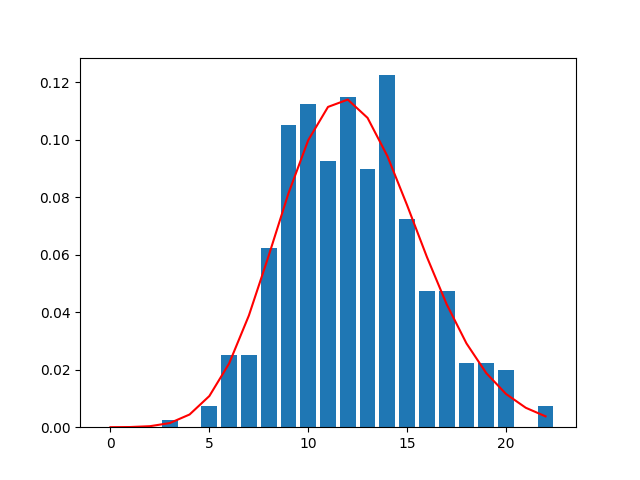
\includegraphics[width=1\textwidth]{10.png}
    \caption{Наложение теоритического распределения Пуасона на экспериментальную диаграмму(для $\tau = 10с$c)}
    \label{fig:my_label}
\end{figure}



\clearpage

\subsection*{При $\tau=20 c$}

\begin{table}[!h]
\begin{center}
\begin{tabular}{|c|c|c|c|c|c|c|c|c|c|c|}
\hline
№Опыта & 1 & 2 & 3 & 4 & 5 & 6 & 7 & 8 & 9 & 10 \\ \hline
0 & 22 & 20 & 27 & 17 & 24 & 21 & 18 & 21 & 24 & 26 \\ \hline
10 & 21 & 27 & 24 & 23 & 24 & 20 & 21 & 22 & 23 & 22 \\ \hline
20 & 18 & 19 & 23 & 25 & 20 & 24 & 36 & 33 & 27 & 27 \\ \hline
30 & 35 & 17 & 26 & 32 & 24 & 23 & 23 & 16 & 17 & 22 \\ \hline
40 & 21 & 31 & 18 & 20 & 20 & 29 & 21 & 27 & 24 & 26 \\ \hline
50 & 21 & 20 & 33 & 24 & 27 & 27 & 30 & 34 & 30 & 22 \\ \hline
60 & 30 & 25 & 18 & 28 & 22 & 17 & 17 & 25 & 25 & 31 \\ \hline
70 & 31 & 28 & 14 & 28 & 29 & 27 & 30 & 24 & 24 & 19 \\ \hline
80 & 27 & 31 & 29 & 31 & 22 & 23 & 28 & 30 & 29 & 18 \\ \hline
90 & 18 & 24 & 25 & 20 & 24 & 19 & 20 & 25 & 23 & 32 \\ \hline
100 & 16 & 25 & 20 & 25 & 21 & 34 & 31 & 23 & 24 & 29 \\ \hline
110 & 23 & 22 & 29 & 24 & 25 & 20 & 28 & 36 & 38 & 25 \\ \hline
120 & 28 & 28 & 25 & 24 & 25 & 24 & 30 & 23 & 17 & 30 \\ \hline
130 & 25 & 29 & 28 & 22 & 22 & 22 & 14 & 25 & 21 & 31 \\ \hline
140 & 17 & 30 & 23 & 20 & 21 & 32 & 28 & 23 & 27 & 22 \\ \hline
150 & 18 & 26 & 29 & 26 & 21 & 24 & 26 & 18 & 24 & 26 \\ \hline
160 & 21 & 37 & 20 & 31 & 20 & 22 & 28 & 27 & 23 & 27 \\ \hline
170 & 22 & 27 & 20 & 22 & 20 & 29 & 27 & 26 & 22 & 19 \\ \hline
180 & 32 & 29 & 28 & 24 & 18 & 25 & 20 & 24 & 28 & 30 \\ \hline
190 & 18 & 29 & 29 & 17 & 28 & 31 & 27 & 21 & 22 & 19 \\ \hline
\end{tabular}
\caption*{Число срабатываний счетчика за $\tau = 20$с}
\end{center}
\end{table}

\begin{table}[!h]
\begin{center}
\begin{tabular}{|c|c|}
\hline
$\langle n\rangle$ & 24.55 \\ \hline
$\sigma_{n}$ & 4.715 \\ \hline
$\sigma_{\langle n\rangle}$ & 0.33 \\ \hline
$j=\frac{\langle n\rangle}{\tau}$ & 1.2275 \\ \hline
$\sigma_{j}$ & 0.017 \\ \hline
\end{tabular}
\end{center}
\end{table}

\begin{figure}[h!]
    \centering
    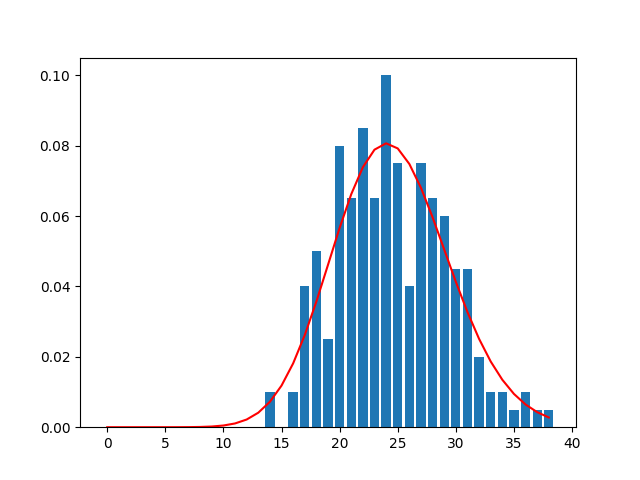
\includegraphics[width=1\textwidth]{20.png}
    \caption{Наложение теоритического распределения Пуасона на экспериментальную диаграмму(для $\tau = 20с$c)}
    \label{fig:my_label}
\end{figure}

Доли случаев, когда отклонение числа отсчётов $n$ от среднего значения не превышает (по модулю):

Одного стандартного отклонения: 0.71
Двух стандартных отклонений: 0.955
Трёх стандартных отклонений: 1.0

\clearpage

\subsection*{При $\tau=40 c$}

\begin{table}[!h]
\begin{center}
\begin{tabular}{|c|c|c|c|c|c|c|c|c|c|c|}
\hline
№Опыта & 1 & 2 & 3 & 4 & 5 & 6 & 7 & 8 & 9 & 10 \\ \hline
0 & 42 & 44 & 45 & 39 & 50 & 48 & 47 & 44 & 43 & 45 \\ \hline
10 & 37 & 48 & 44 & 69 & 54 & 52 & 58 & 47 & 39 & 39 \\ \hline
20 & 52 & 38 & 49 & 48 & 50 & 41 & 57 & 54 & 64 & 52 \\ \hline
30 & 55 & 46 & 39 & 42 & 56 & 59 & 42 & 56 & 54 & 43 \\ \hline
40 & 58 & 60 & 45 & 58 & 47 & 42 & 45 & 43 & 45 & 55 \\ \hline
50 & 41 & 45 & 55 & 54 & 53 & 45 & 53 & 45 & 64 & 63 \\ \hline
60 & 56 & 49 & 49 & 53 & 47 & 54 & 50 & 44 & 39 & 52 \\ \hline
70 & 47 & 43 & 53 & 51 & 49 & 44 & 55 & 45 & 44 & 50 \\ \hline
80 & 58 & 51 & 42 & 55 & 50 & 49 & 42 & 49 & 53 & 41 \\ \hline
90 & 61 & 52 & 43 & 44 & 58 & 47 & 46 & 59 & 48 & 41 \\ \hline
\end{tabular}
\caption*{Число срабатываний счетчика за $\tau = 40$с}
\end{center}
\end{table}

\begin{table}[!h]
\begin{center}
\begin{tabular}{|c|c|}
\hline
$\langle n\rangle$ & 49.1 \\ \hline
$\sigma_{n}$ & 6.66 \\ \hline
$\sigma_{\langle n\rangle}$ & 0.67 \\ \hline
$j=\frac{\langle n\rangle}{\tau}$ & 1.2275 \\ \hline
$\sigma_{j}$ & 0.017 \\ \hline
\end{tabular}
\end{center}
\end{table}

Доли случаев, когда отклонение числа отсчётов $n$ от среднего значения не превышает (по модулю):

Одного стандартного отклонения: 0.66
Двух стандартных отклонений: 0.96
Трёх стандартных отклонений: 1.0

\begin{figure}[h!]
    \centering
    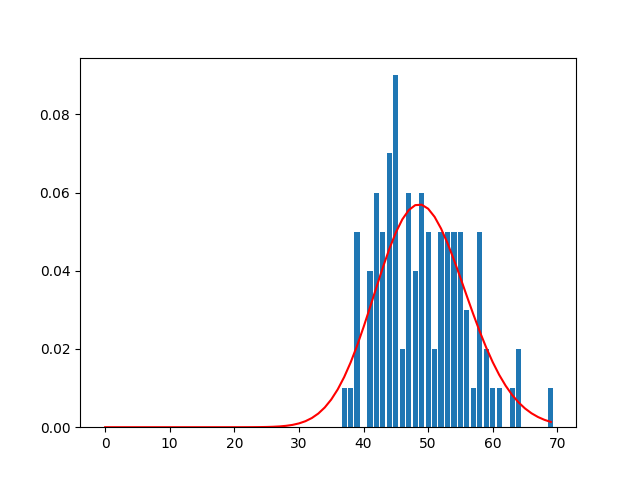
\includegraphics[width=1\textwidth]{40.png}
    \caption{Наложение теоритического распределения Пуасона на экспериментальную диаграмму(для $\tau = 40$c)}
    \label{fig:my_label}
\end{figure}

\clearpage

\subsection*{При $\tau=80 c$}

\begin{table}[!h]
\begin{center}
\begin{tabular}{|c|c|c|c|c|c|c|c|c|c|c|}
\hline
№Опыта & 1 & 2 & 3 & 4 & 5 & 6 & 7 & 8 & 9 & 10 \\ \hline
0 & 86  & 84  & 98  & 91  & 88  & 85  & 113 & 106 & 105 & 78  \\ \hline
10 & 90  & 97  & 91  & 111 & 116 & 101 & 81  & 115 & 98  & 97  \\ \hline
20 & 118 & 103 & 89  & 88  & 100 & 86  & 109 & 98  & 98  & 127 \\ \hline
30 & 105 & 102 & 101 & 94  & 91  & 90  & 104 & 93  & 100 & 94  \\ \hline
40 & 109 & 97  & 99  & 91  & 94  & 113 & 87  & 105 & 105 & 89 \\ \hline
\end{tabular}
\caption*{Число срабатываний счетчика за $\tau = 80$с}
\end{center}
\end{table}

\begin{table}[!h]
\begin{center}
\begin{tabular}{|c|c|}
\hline
$\langle n\rangle$ & 98.2 \\ \hline
$\sigma_{n}$ & 10.298 \\ \hline
$\sigma_{\langle n\rangle}$ & 1.46 \\ \hline
$j=\frac{\langle n\rangle}{\tau}$ & 1.2275 \\ \hline
$\sigma_{j}$ & 0.017 \\ \hline
\end{tabular}
\end{center}
\end{table}

Доли случаев, когда отклонение числа отсчётов $n$ от среднего значения не превышает (по модулю):

Одного стандартного отклонения: 0.68
Двух стандартных отклонений: 0.98
Трёх стандартных отклонений: 1.0

\begin{figure}[h!]
    \centering
    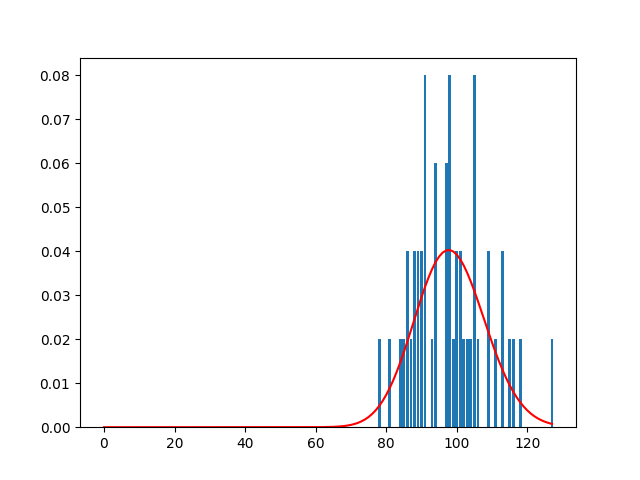
\includegraphics[width=1\textwidth]{80.png}
    \caption{Наложение теоритического распределения Пуасона на экспериментальную диаграмму(для $\tau = 80$c)}
    \label{fig:my_label}
\end{figure}

\clearpage

\section*{Обсуждение результатов}

Можно заметить, что средняя интенсивность регистрируемых частиц в секунду не зависит от величины интервала $\tau$ и числа точек $N=\frac{t}{\tau}$

Экспериментальные гистограммы с большой точностью согласуются с распределением Пуассона.

Основное свойство распределения Пуассона выполняется с точностью до десятых. Можно сделать вывод, что регистрация частиц является однородным во времени случайным процессом, а количество
отсчётов в одном опыте подчиняется распределению Пуассона.

Можно сделать вывод, что при достаточно больших $\overline{n}$ распределение Пуассона приближается к нормальному распределению (распределению Гаусса)

\section*{Вывод}

В ходе выполнения работы познакомился с основными понятиями статистики. Определил среднее число регистрируемых космических лучей в секунду и определил погрешность результата. Выяснил, что средняя интенсивность регистрируемых частиц в секунду не зависит от величины интервала $\tau$ и числа точек $N = \frac{t}{\tau}$ . Проверил возможность описания исследуемого процесса статистическими законами Пуассона и Гаусса.


\end{document}